\chapter{原理与实现}\label{chapter:implementation}
分布式二级哈希表是一个偏向工程的项目,涉及到的大多是已经发展成熟的技术,是对分
布式领域一些经典算法的综合。但是分布式二级哈希表对系统的运行效率要求很高,因此
要求在实现细节上不能有瑕疵。本章是论文中篇幅最大的一章,一方面详细阐述了分布式
二级哈希表用到的经典技术的原理,另一方面也深入说明系统的实现细节。

对于像分布式二级哈希表这样并不复杂的系统,在实现时仍然体现了模块化的思想,整个
系统是由一系列模块搭建而成的。每个模块完成特定的功能,基本独立,但是在实现时也
要考虑模块之间的协作关系。这些模块有些是由我独立实现的,有些在实现时参考了别人
的代码,有些将别人的代码加以修改后移植到系统里来,有些则直接使用了别人的代码。
所有的引用和参考都基于开源代码,并且符合作者的协议和使用条款。

分布式二级哈希表的所有模块都用标准C语言写成。相比与其他的脚本语言或者面向对象
编程语言,C语言有着更高的执行效率。C语言的灵活度比较高,对于像分布式二级哈希表
这样对系统执行效率要求颇高的工程,用C语言开发有更大的优化自由度。由于C++语言可
以兼容C语言,但反之不行,所以C语言有更高的可移植性。由于存储服务器上运行的都是
Linux系统,C语言无疑是最佳的选择,所以我决定选用标准C语言实现分布式二级哈希表
的全部开发。另一方面,相比C++语言和其他面向对象编程语言,C语言的标准库和第三方
库都不够丰富,这也迫使我自己实现了像线程池这样的模块,反而锻炼了自己的编程能
力。

下面我将分模块详细阐述每一部分的原理和实现细节。

\section{配置服务器}
配置服务器是整个分布式二级哈希表的核心。它通过与集群中每一个存储服务器进行心跳
通信,掌控集群中所有结点的运转情况。配置服务器实现了一致性哈希算法,负责决定数
据如何在存储结点间进行分配和备份。当上层应用调用系统的接口函数时,客户端首先通
过远程过程调用,从配置服务器获取目标数据所有副本所处服务器的IP地址。在当前的系
统设计中,由于数据已经有多份备份,并且机器故障发生概率很低,所以配置服务器忽略
可能发生的单个结点故障。如果希望配置服务器能够解决存储结点动态加入和离开集群的
情况,需要在当前的系统实现上添加数据迁移模块。

\subsection{一致性哈希算法}\label{subsection:consistent}
一致性哈希算法自诞生之日起,就因其优雅的设计而备受青睐,并且被众多著名分布式存
储系统所采纳。一致性哈希算法的优势在于,当存储结点动态增多和减少时,需要在结点
间转移的数据量最小。虽然分布式二级表的当前设计并不支持结点的动态加入和移除,但
是为了增强系统的可扩展性,我仍然采用了一致性哈希算法来解决数据分配和备份问题。

下面先介绍一致性哈希算法的原理。将哈希函数作用于数据的索引空间,得到的值域空间
称作\emph{哈希空间}。将哈希空间首尾相接,回绕成一个环状空间,称作
\emph{哈希环},如图\ref{figure:consistent}所示。每一个索引的哈希值在哈希环上有
唯一的一个点与之对应,我们用这个点代表具有这个索引的数据。每一个存储结点被称作
一个\emph{物理结点},使用某个字符串作为其唯一标识,比如IP地址。每一个物理结点
有若干\emph{虚拟结点}与之对应,虚拟结点数一般设定为与物理结点的存储容量成正
比。每一个虚拟节点也有一个唯一的字符串标识,一般通过在其对应物理节点的标识后面
附加结点编号构成。图\ref{figure:consistent}中,画出了两个物理结点,其中一个物
理节点画出了两个虚拟结点(深灰色),另一个物理结点只画出了一个虚拟结点(浅灰色
)。将所有虚拟节点的字符串标识求哈希值,结果也是哈希环上的一点,我们用这个点代
表这个虚拟节点对应的物理结点。这样,一个物理结点有几个虚拟结点与之对应,哈希环
上就有几个点与这个物理结点对应。由于哈希函数的性质,与某个物理结点对应的那些点
在哈希环上的分布并无规律可循,当物理结点包含足够多的虚拟结点时,这些点可以看作
是随机分布的。后面我们会看到,正是这个性质保证了一致性哈希在结点动态加入和移出
时,数据迁移量最小。
\begin{figure}
  \centering
  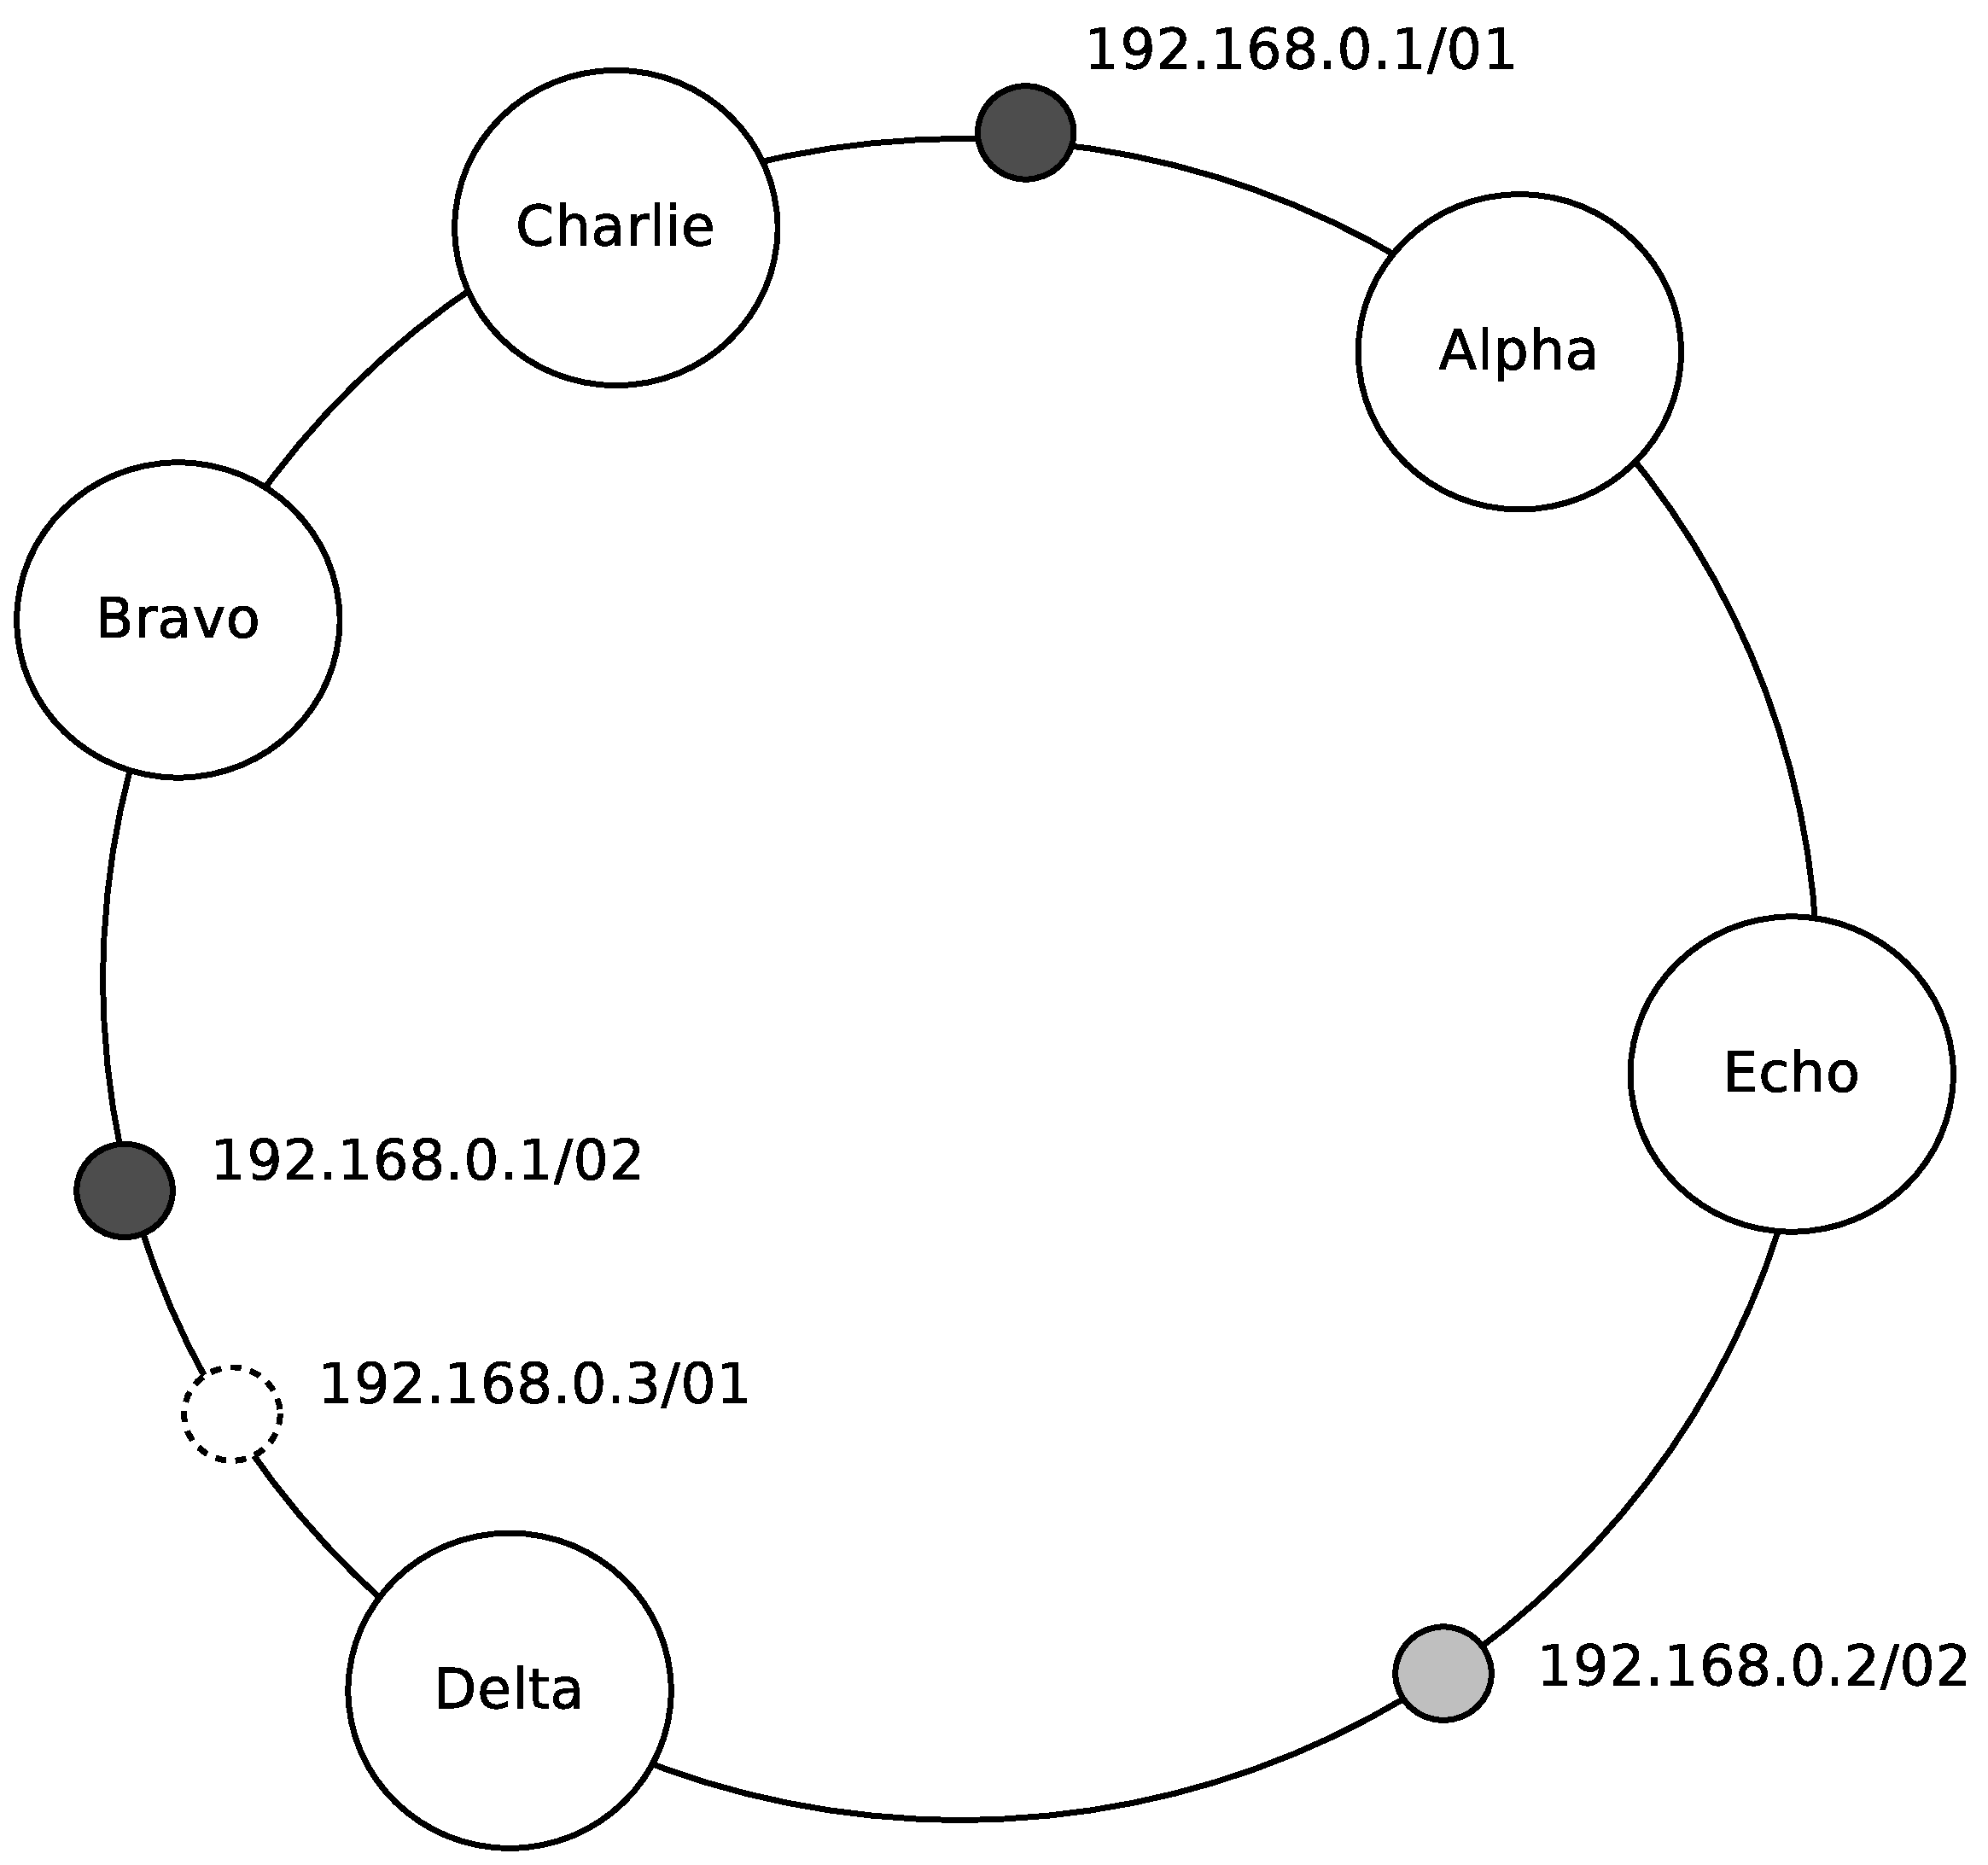
\includegraphics[width=0.8\linewidth]{consistent}
  \caption[一致性哈希算法]{一致性哈希算法。最大的圆环是哈希环。在哈希环上,标
  有字母的大圆代表数据,上面的单词是该数据的索引,图中画出了五个数据。哈希环上
  的小圆代表虚拟结点,旁边标注的字符串是该虚拟结点的标识,同样灰度的小圆对应相
  同的物理结点。系统稳定时有两个物理结点,IP地址为192.168.0.1的物理结点配置了
  两个虚拟结点,用深灰色小圆表示;IP地址为192.168.0.2的物理结点配置了一个虚拟
  结点,用浅灰色小圆表示。对于任何一个数据,其索引的哈希值在哈希环上有唯一的一
  点与之对应。从该点开始,顺着哈希环沿逆时针方向找到M个虚拟结点,这M个结点对应
  的N个不同物理结点即存放该数据的存储服务器,N为数据在系统中的副本数。当系统中
  有新的结点加入,如虚线小圆表示的IP地址为192.168.0.3的存储服务器,假设N等于
  1,需要迁移的数据只有那些索引的哈希值落到从浅灰色虚拟结点到新加入虚拟结点之
  间的劣弧上的数据,这些数据将从深灰色虚拟结点对应的物理结点上移动到新加入的物
  理结点上,即索引值为Delta的数据将从IP地址为192.168.0.1的存储结点上移动到新加
  入的IP地址为192.168.0.3的存储结点上。除此之外,索引的哈希值落在从新加入的虚
  拟结点到浅灰色虚拟结点的优弧上的所有数据都不必做出移动。期望的数据移动量为
  系统中数据总量的(C + 1)分之一,C为结点加入前集群的规模,这也是在保证系统存储
  负载平衡的前提下,任何算法所能达到的数据迁移量下界。此外,一致性哈希算法保证
  了集群中存在结点动态变化时,变化前后系统的存储负载都是均衡的。}
  \label{figure:consistent}
\end{figure}

现在我们有了一个哈希环;对每一个数据的索引求哈希后,在哈希环上都有一点和这个数
据对应;对于集群中的每一台存储服务器,在哈希环上都有若干点与之对应,并且这些点
是随机分布的。在图\ref{figure:consistent}中,最大的圆环是哈希环。在哈希环上,
标有字母的大圆代表数据,上面的单词是该数据的索引。哈希环上的小圆代表虚拟结点,
旁边标注的字符串是该虚拟结点的唯一标识。同样灰度的小圆对应相同的物理结点。那么
如何决定数据的分配和备份呢?一致性哈希算法规定,对于任何一个数据,将哈希函数作
用在它的索引之上,得到的哈希值在哈希环上有唯一一点与之对应。从该点开始,顺着哈
希环沿逆时针方向会找到M个虚拟结点。如果这M个虚拟结点对应N个不同物理结点(N为数
据在整个系统中的副本数,并且显然N不大于M),那么该数据就应当存放在这N个物理结
点上。在图\ref{figure:consistent}中,假设N等于1,那么索引为Alpha的数据应当存放
在IP地址为192.168.0.2的物理结点上,索引为Bravo的数据应当存放在IP地址为
192.168.0.1的物理结点上;如果N等于2,那么图中画出的所有数据都应当在两台服务器
上各存放一个副本。

另一种决定数据在存储服务器之间分配的方法,在实现上比一致性哈希算法简单。首先对
集群中的C台机器从0到C-1依次编号。对于每一个数据,计算其索引的哈希值。由于数据
在计算机中的最终表示是二进制,所以哈希值也可以当成一个整数来处理。将这个整数除
以C,得到的余数即为N等于1时,应当存储该数据的服务器的编号。对于N大于1的情形,
只需要找到编号不小于该余数的连续N台服务器即可。\footnote{如果超过C-1则从0开始
数}这种\emph{除留余数法}与一致性哈希算法相比,思路更加直观,实现也方便,对于集
群结点固定的系统,不失为一种理想的解决方案。

但是在大型的数据中心里,集群规模一般为几千台甚至更多的服务器,结点故障不是偶尔
发生,而是可能一直存在。这要求有一种算法能够应对结点的动态加入和移出,将这种变
化造成的数据迁移量降至最低。对于除留余数法,假设集群中总数据量为D,当有一个新
存储结点加入原本规模为C的集群,那么需要迁移的数据量由公式\ref{equation:modula}
计算得:
\begin{equation}\label{equation:modula}
(\frac{D}{C} - \frac{D}{C - 1}) * (1 + 2 + \dots + (C - 1)) = \frac{D}{2}
\end{equation}
也就是说,当有一个结点动态加入集群时,平均有一半的数据要从原存储服务器移动到另
一台服务器。结点移出集群是加入的逆过程,所有当有一个结点因为故障而不再正常运转
时,平均有一半的数据将发生转移。当结点故障异常频繁时,这种数据迁移规模将耗费大
量的网络带宽和硬盘读写能力,对分布式存储系统将是一个极大的负担。

再回到一致性哈希算法。假设系统稳定后有一个新的存储服务器加入了集群,并且它设置
了一个虚拟结点,如图\ref{figure:consistent}中虚线小圆所示。当N等于1时,需要迁
移的数据只有那些索引的哈希值落到从浅灰色虚拟结点到新加入虚拟结点之间的劣弧上的
数据,这些数据将从深灰色虚拟结点对应的物理结点上移动到新加入的物理结点上,即索
引值为Delta的数据将从IP地址为192.168.0.1的存储结点上移动到新加入的IP地址为
192.168.0.3的存储结点上。除此之外,索引的哈希值落在从新加入的虚拟结点到浅灰色
虚拟结点的优弧上的所有数据都不必做出移动。当N大于1时,情况与之类似,请读者以图
\ref{figure:consistent}为例自行判断哪些数据应该做出移动。那么系统中需要移动的
数据总量是多少呢?考虑结点加入的逆过程,即有一个结点离开集群,需要移动的所有数
据就是这个结点原先负责存储的所有数据。由于每个物理结点对应很多的虚拟结点,而这
些虚拟结点又是随机分布的,因此在结点离开集群之前,数据在集群中的分布是近似平均
的。也就是说,规模为C的集群,一个结点动态离开带来的数据迁移量是$\frac{D}{C}$,
一个结点动态加入造成的数据迁移量是$\frac{D}{C + 1}$。显然这两个数值是在保证系
统存储负载均衡的性质下,数据迁移量的下界。因而当结点动态移入和移出系统时,一致
性哈希算法在数据迁移量方面是最优的算法,并且达到了理论下界。一致性哈希算法的另
一个优点是在集群中结点动态变化时,它仍然保持了系统存储负载均衡的性质。前面已经
分析过,当系统稳定时,一致性哈希算法保证了存储负载均衡。当某个物理结点离开集群
后,原先那些由它某个虚拟结点负责的数据,将被这个虚拟结点按顺时针方向看的下一个
虚拟结点所承担。由于物理结点的所有虚拟结点是随机分布的,那么当一个物理结点对应
足够多的虚拟结点时,这些被选中的虚拟结点将以相同的数目对应全部的物理结点。换句
话说,原先由那个离开的物理结点负责的数据将被平均分成若干份,集群中其余的每个物
理结点将得到相同的份数,所以得到的数据总量也相同。因此,一致性哈希算法保证了集
群中存在结点动态变化时,变化前后系统的存储负载都是均衡的。

分布式二级哈希表的配置服务器实现了一致性哈希算法。开源项目libconhash是一个用标
准C语言写就的,能在Windows和Linux平台下运行的一致性哈希算法实现。但是它不支持
在系统中进行数据备份,并且其中一些功能的实现策略不适合分布式二级哈希表。因此我
在原工程的框架下重写了部分代码,添加了诸多功能,比如使得系统可以支持数据备份,
最终将其成功移植到分布式二级哈希表系统中来。

在分布式二级哈希表中,由于系统设计不予考虑结点动态加入和离开的情形,因此配置服
务器通过读取配置文件获取集群中所有存储服务器的主机名或IP地址。由于集群中各存储
结点是同构的,因此直接设定每个物理结点对应1024个虚拟结点。哈希函数选用128位MD5
哈希\cite{rivest1992rfc1321},保证了虚拟结点在哈希环上的随机分布性质。

实现一致性哈希的另一个关键点是如何在哈希环上快速找到顺时针方向下一个虚拟结点。
由于C语言的标准库中不具有像Java语言中HashMap那样的数据结构可以直接调用实现此功
能的接口函数,在分布式二级哈希表中,这个问题通过自己实现了一棵红黑树
\footnote{http://en.wikipedia.org/wiki/Red-black\_tree}来解决。红黑树是一种平
衡二叉搜索树,它具有以下性质:
\begin{enumerate}
  \item 结点被涂以红色或者黑色。
  \item 根结点被涂以黑色。
  \item 所有叶结点被涂以黑色。
  \item 所有红色结点的左右子结点都被涂以黑色。
  \item 给定一个结点,从这个结点开始到它任何一个后代叶结点的所有路径包含相同数
  目的黑色结点。
\end{enumerate}
这些性质保证了红黑树是一棵基本平衡的二叉树,在它上面进行搜索的最差时间复杂度为
O(log(N)),其中N为红黑树中结点的个数。在分布式二级哈希表中,所有的虚拟结点都有
一个在红黑树中的叶子结点与之对应,排序依据就是这个虚拟结点的标识字符串的MD5
值。当我们需要查看一个某个数据存储在哪些物理结点上时,就把这个数据的索引取MD5
值,再拿这个值在红黑树中去搜索,找到第一个哈希值不小于这个值的虚拟结点,再从这
个虚拟结点的哈希值开始,往后找N - 1个哈希值严格增大,并且对应不同物理结点的虚
拟结点。如果在这个过程中需要找比某个值大的虚拟结点,但是这个值比红黑树中最大的
哈希值还大,那么直接返回哈希值最小的那个虚拟结点。给定索引确定数据所在存储服务
器的IP地址的函数伪代码如下:
\begin{code}
  FUNC getIpsByKey(IN string key, IN int N, OUT IP[] ips)
  {
    GLOBE RBTREE rbtree;
    VAR VNODE vnode, start;

    vnode = rbtree.geq( MD5(key) );
    ips[0] = vnode.node.ip;
    start = vnode;
    for i from 1 to (N - 1)
    {
1:    vnode = rbtree.ge( vnode.hash );
      if ( vnode == start ) ERROR;
      for j from 0 to i - 1
      {
        if ( ips[j] == vnode.node.ip ) goto 1;
      }
      ips[i] = vnode.node.ip;
    }
  }
\end{code}
前面我们说到在红黑树中搜索的时间复杂度为O(log(N)),其中N为树中结点总个数。在分
布式二级哈希表的一致性哈希实现中,红黑树中的结点数就是系统中虚拟结点的总数。在
第\ref{section:assumption}节中的一个假设是系统的典型规模为50台存储服务器,按照
上文提到的每个物理结点配置1024个虚拟结点计算,一次查询需要花费的时间规模与处理
器进行16次运算相当,因此用红黑树实现一致性哈希具有很高的查询效率。

此外,之前在原理介绍中提到的数据索引,在分布式二级哈希表的实现中,指的是blob的
bucketID。也就是说,同一个桶中的blob将存储在相同的服务器上。一致性哈希算法对于
数据的分配粒度是相对于桶的,它不能区分同一个桶中不同的blob。在这种情况下,集群
的存储负载平衡是由另一个假设保证的。即我们假设单个blob较小,但是blob和桶的个数
很多。如果我们将桶中所有blob的大小求和作为桶的大小,那么虽然桶的大小可能差异很
大,但是由于每个物理结点都存储了很多的桶,而且这些桶是随机分配的,那么当桶的数
目足够多时,每个物理结点的总存储量是近似相同的。

\subsection{远程过程调用}
除了一致性哈希算法,配置服务还包含另一个重要模块,即远程过程调用模块。在分布式
二级哈希表中,客户端通过远程过程调用从配置服务器获取某个数据所在的目标存储服务
器的IP地址。

远程过程调用是一种客户端和服务器交互的技术,它使得客户端程序可以调用执行在远端
服务器上的一段程序,而调用方法就好像在执行本地的函数一样,不必客户端和服务器的
网络交互,以及其他实现细节。分布式二级哈希表采用ONC RPC
\footnote{http://en.wikipedia.org/wiki/ONC\_RPC}标准规定的远程过程调用协议,代
码执行流如图\ref{figure:oncrpc}所示。客户端执行callrpc系统调用,并将参数按照本
地函数调用的方式压栈。callrpc从中提取出目标服务器例程的信息,并将该例程需要的
参数按照事先定义的方式打包,然后通过TCP或UDP协议将参数发送至指定服务器。目标服
务器事先已经注册了一段例程,并监听ONC RPC使用的默认端口111。一旦收到客户端发来
的打包数据,按照事先定义的方式从中提取出参数,并传递给服务器例程。接着服务器例
程在用户态执行,执行完毕后,进入内核态,由操作系统将返回值按照事先约定的方式打
包,再依照相同的传输层协议,通过刚才建立的连接,将打包后的返回值传回客户端。至
此,此次远程过程调用服务器端的工作完成,服务器端准备应答下一个请求。客户端收到
服务器发送来的打包数据,按照事先约定的方式从中提取出返回值。然后callrpc系统调
用返回,将远程过程调用的返回值传递给用户态的客户端主程序,本次远程过程调用执行
完毕。
\begin{figure}
  \centering
  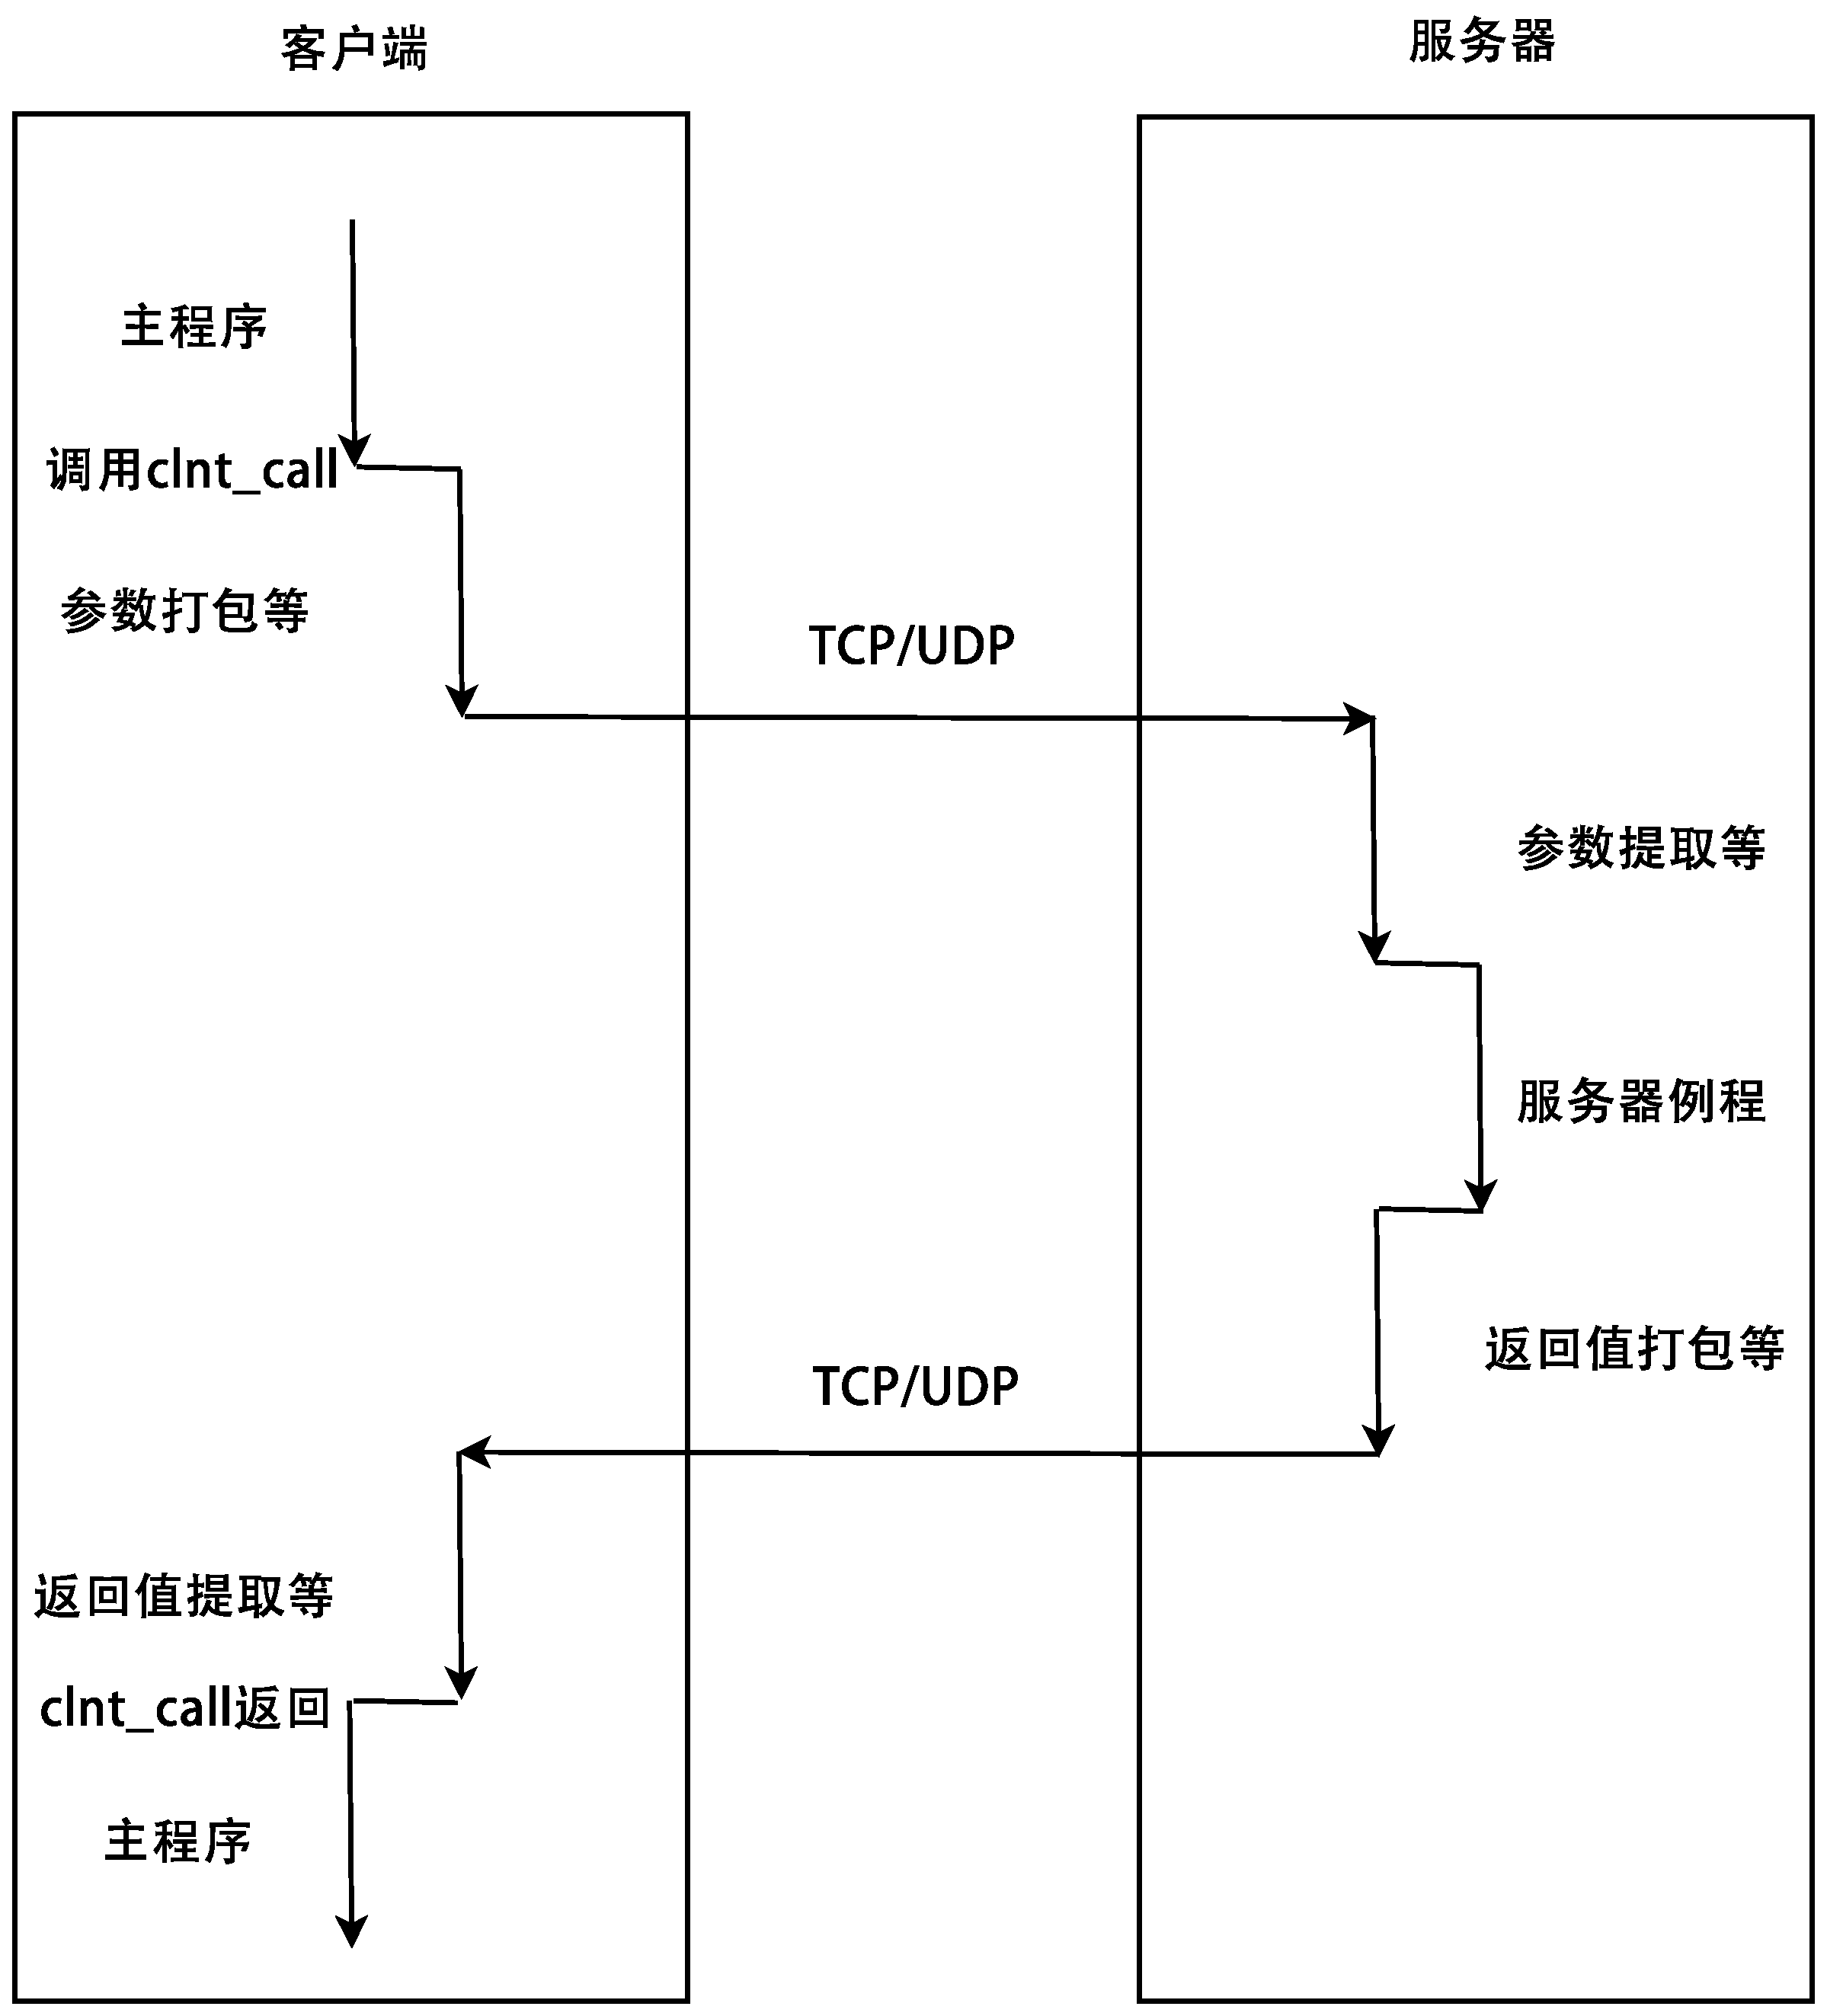
\includegraphics[width=1.0\linewidth]{oncrpc}
  \caption[ONC RPC代码执行流]{ONC RPC代码执行流。客户端用户态主程序执行
  callrpc系统调用。callrpc将服务器目标例程需要的参数按照事先定义的方式打包,然
  后通过TCP或UDP协议将打包数据发送至指定服务器。目标服务器事先已经注册了一段例
  程,并监听ONC RPC使用的默认端口111。收到客户端发来的打包数据后按照事先定义的
  方式从中提取出参数,并传递给用户态服务器例程。服务器例程执行完毕后,进入内核
  态,由操作系统将返回值按照事先约定的方式打包,再通过刚才建立的连接将打包后的
  返回值传回客户端。至此,此次远程过程调用服务器端工作完成,端准备应答下一个请
  求。客户端收到服务器发送来的数据,按照事先约定的方式从中提取返回值。然后
  callrpc返回,将远程过程调用的返回值传递给用户态的客户端主程序,本次远程过程
  调用执行完毕。}
  \label{figure:oncrpc}
\end{figure}

远程过程调用这种客户端和服务器的交互机制,简化了程序员的变成,其中,参数和返回
值的打包,数据在客户端和服务器之间的可靠性传输等工作均由系统来实现。但是,上述
代码执行流程对于纯粹写应用的程序员仍然略显复杂,比如,程序员需要\emph{告知}系
桶如何对数据进行打包和提取,需要初始化网络参数等。为了进一步简化程序员编程,使
程序员将主要精力放在将要实现的功能上,而不是远程过程调用本身的实现上,编程工具
rpcgen\footnote{http://en.wikipedia.org/wiki/Rpcgen}应运而生。程序员只需要书写
一个简单的配置文件,声明服务器例程的原型,以及各参数和返回值的数据结构,rpcgen
就能据此产生出服务器和客户端将要用到的全部C代码。程序员只需要在服务器端例程的
框架里填入具体实现,再将客户端代码和服务器端代码分别编译,便实现了远程过程调
用。比如,在分布式二级哈希表中,客户端通过远程过程调用,给定一个索引,从配置服
务器得到具备这个索引的数据所在的存储服务器的IP地址。那么rpcgen的配置文件
cfgsrv.x内容非常简单:
\begin{code}
typedef u_int ips<>;

program CFGSRVPROG {
  version CFGSRVVERS {
    ips GET_HOSTS_BY_KEY(string) = 1;
  } = 1;
} = 1;
\end{code}
其中指定了服务器端例程的原型。参数只有一个,即字符串类型的索引值。返回值是无符
号类型整数的可变长度数组,其中每个元素是一个目标存储服务器的IP地址。rpcgen据此
生成了四个文件:
\begin{enumerate}
  \item cfgsrv.h: 基本的声明文件。编译客户端和服务器端程序时都需要引入此头文
  件。
  \item cfgsvr\_clnt.c: 客户端辅助文件,以实现远程过程调用机制,其中只定义了一
  个函数get\_hosts\_by\_key\_1。客户端主程序调用这个本地函数,就能从配置服务器
  获取目标存储服务器的IP地址。
  \item cfgsrv\_svc.c: 服务器端辅助文件,以实现远程过程调用机制。
  \item cfgsrv\_xdr.c: 服务器端例程的参数和返回值打包程序。
\end{enumerate}
为了完成远程过程调用机制,服务器端还需要实现cfgsrv.h中声明的
get\_hosts\_by\_key\_1和get\_hosts\_by\_key\_1\_svc两个函数。其中第一个函数是
服务器端真正完成通过索引获取目标存储服务器IP地址的例程,可以调用第
\ref{subsection:consistent}小节介绍的一致性哈希算法的实现函数。第二个函数只是
对第一个函数的包装。之后通过rpcgen -m命令可以得到服务器端初始化远程过程调用的
代码。至此,将上述文件合理编译,即可得到实现了远程过程调用的服务器和客户端模
块。

远程过程调用简化了客户端和服务器端实现通信的机制。如果不使用远程过程调用,一种
实现方式是直接在客户端和服务器端建立TCP/UDP连接,再按照自定义的协议传送数据。
在第\ref{section:assumption}实验假设中提到分布式二级哈希表平均每台服务器每秒处
理的请求数不小于50,平均响应时间为百毫秒数量级,这说明客户端一直会发起大量的请
求。如果每一个请求完成之后都关闭socket连接,下个请求到来时再重新建立连接,那么
创建socket和回收资源的系统开销将会非常大,严重影响系统运行性能。这要求每个客户
端和配置服务器的socket连接一直持续,直到客户端程序全部运行结束。基于这个前提,
由于要保证系统的平均响应时间和吞吐量,请求必须设定为异步的,而不能像同步系统那
样将请求放置在一个队列里,在上一个请求结束之后再处理下一个请求。因此,请求的返
回顺序可能和发起顺序不同,客户端可能先收到后发出的请求的返回值,再收到先发出的
请求的返回值。在同一个socket连接中,客户端需要为每个请求附上一个唯一的流水号,
服务器则要为返回值贴上相同的流水号。另一方面,在编程实现上,异步请求也较同步请
求更为复杂,容易出错且不易调试。如果维护返回值和请求的对应关系,以及请求的异步
化都由远程过程调用的框架来完成,那么对于程序员来说,客户端的每次请求就是对本地
函数的一次调用,不必过多考虑上述实现细节。

\section{客户端}\label{section:client}
在第\ref{chapter:architecture}章中曾介绍过,分布式二级哈希表中的客户端是一个独
立的模块,是分布式二级哈希表的一个函数库,上层应用需要将这些代码编译到可执行文
件中去。客户端直接从配置服务器拿到目标存储服务器的IP地址,再与这些服务器进行通
信,执行操作,并将返回值传递给上层应用。这样,完成一次操作总共需要进行两次网络
通信。第一次是客户端通过远程过程调用从配置服务器拿到路由信息,第二次是客户端将
请求发送给具体的存储结点,得到返回值。这种决策的缺点是上层应用需要嵌入分布式二
级哈希表的标准C代码,降低了分布式二级哈希表的易用性和通用性。另一种不许要嵌入
系统框架代码的解决方案是,让客户端直接与某一台入口服务器按照某种协议进行通信,
再有这台入口服务器完成客户端的功能。这样入口服务器和客户端之间还要多进行一次网
络通信,势必增加请求的平均响应时间,并且消耗网络带宽。由于分布式二级哈希表更在
意系统的运行效率,而且上层应用是由我们自己搭建的,因此最终我选用了第一种方案来
实现客户端。

客户端采用了分层结构,如图\label{figure:client}所示。
\begin{figure}
  \centering
  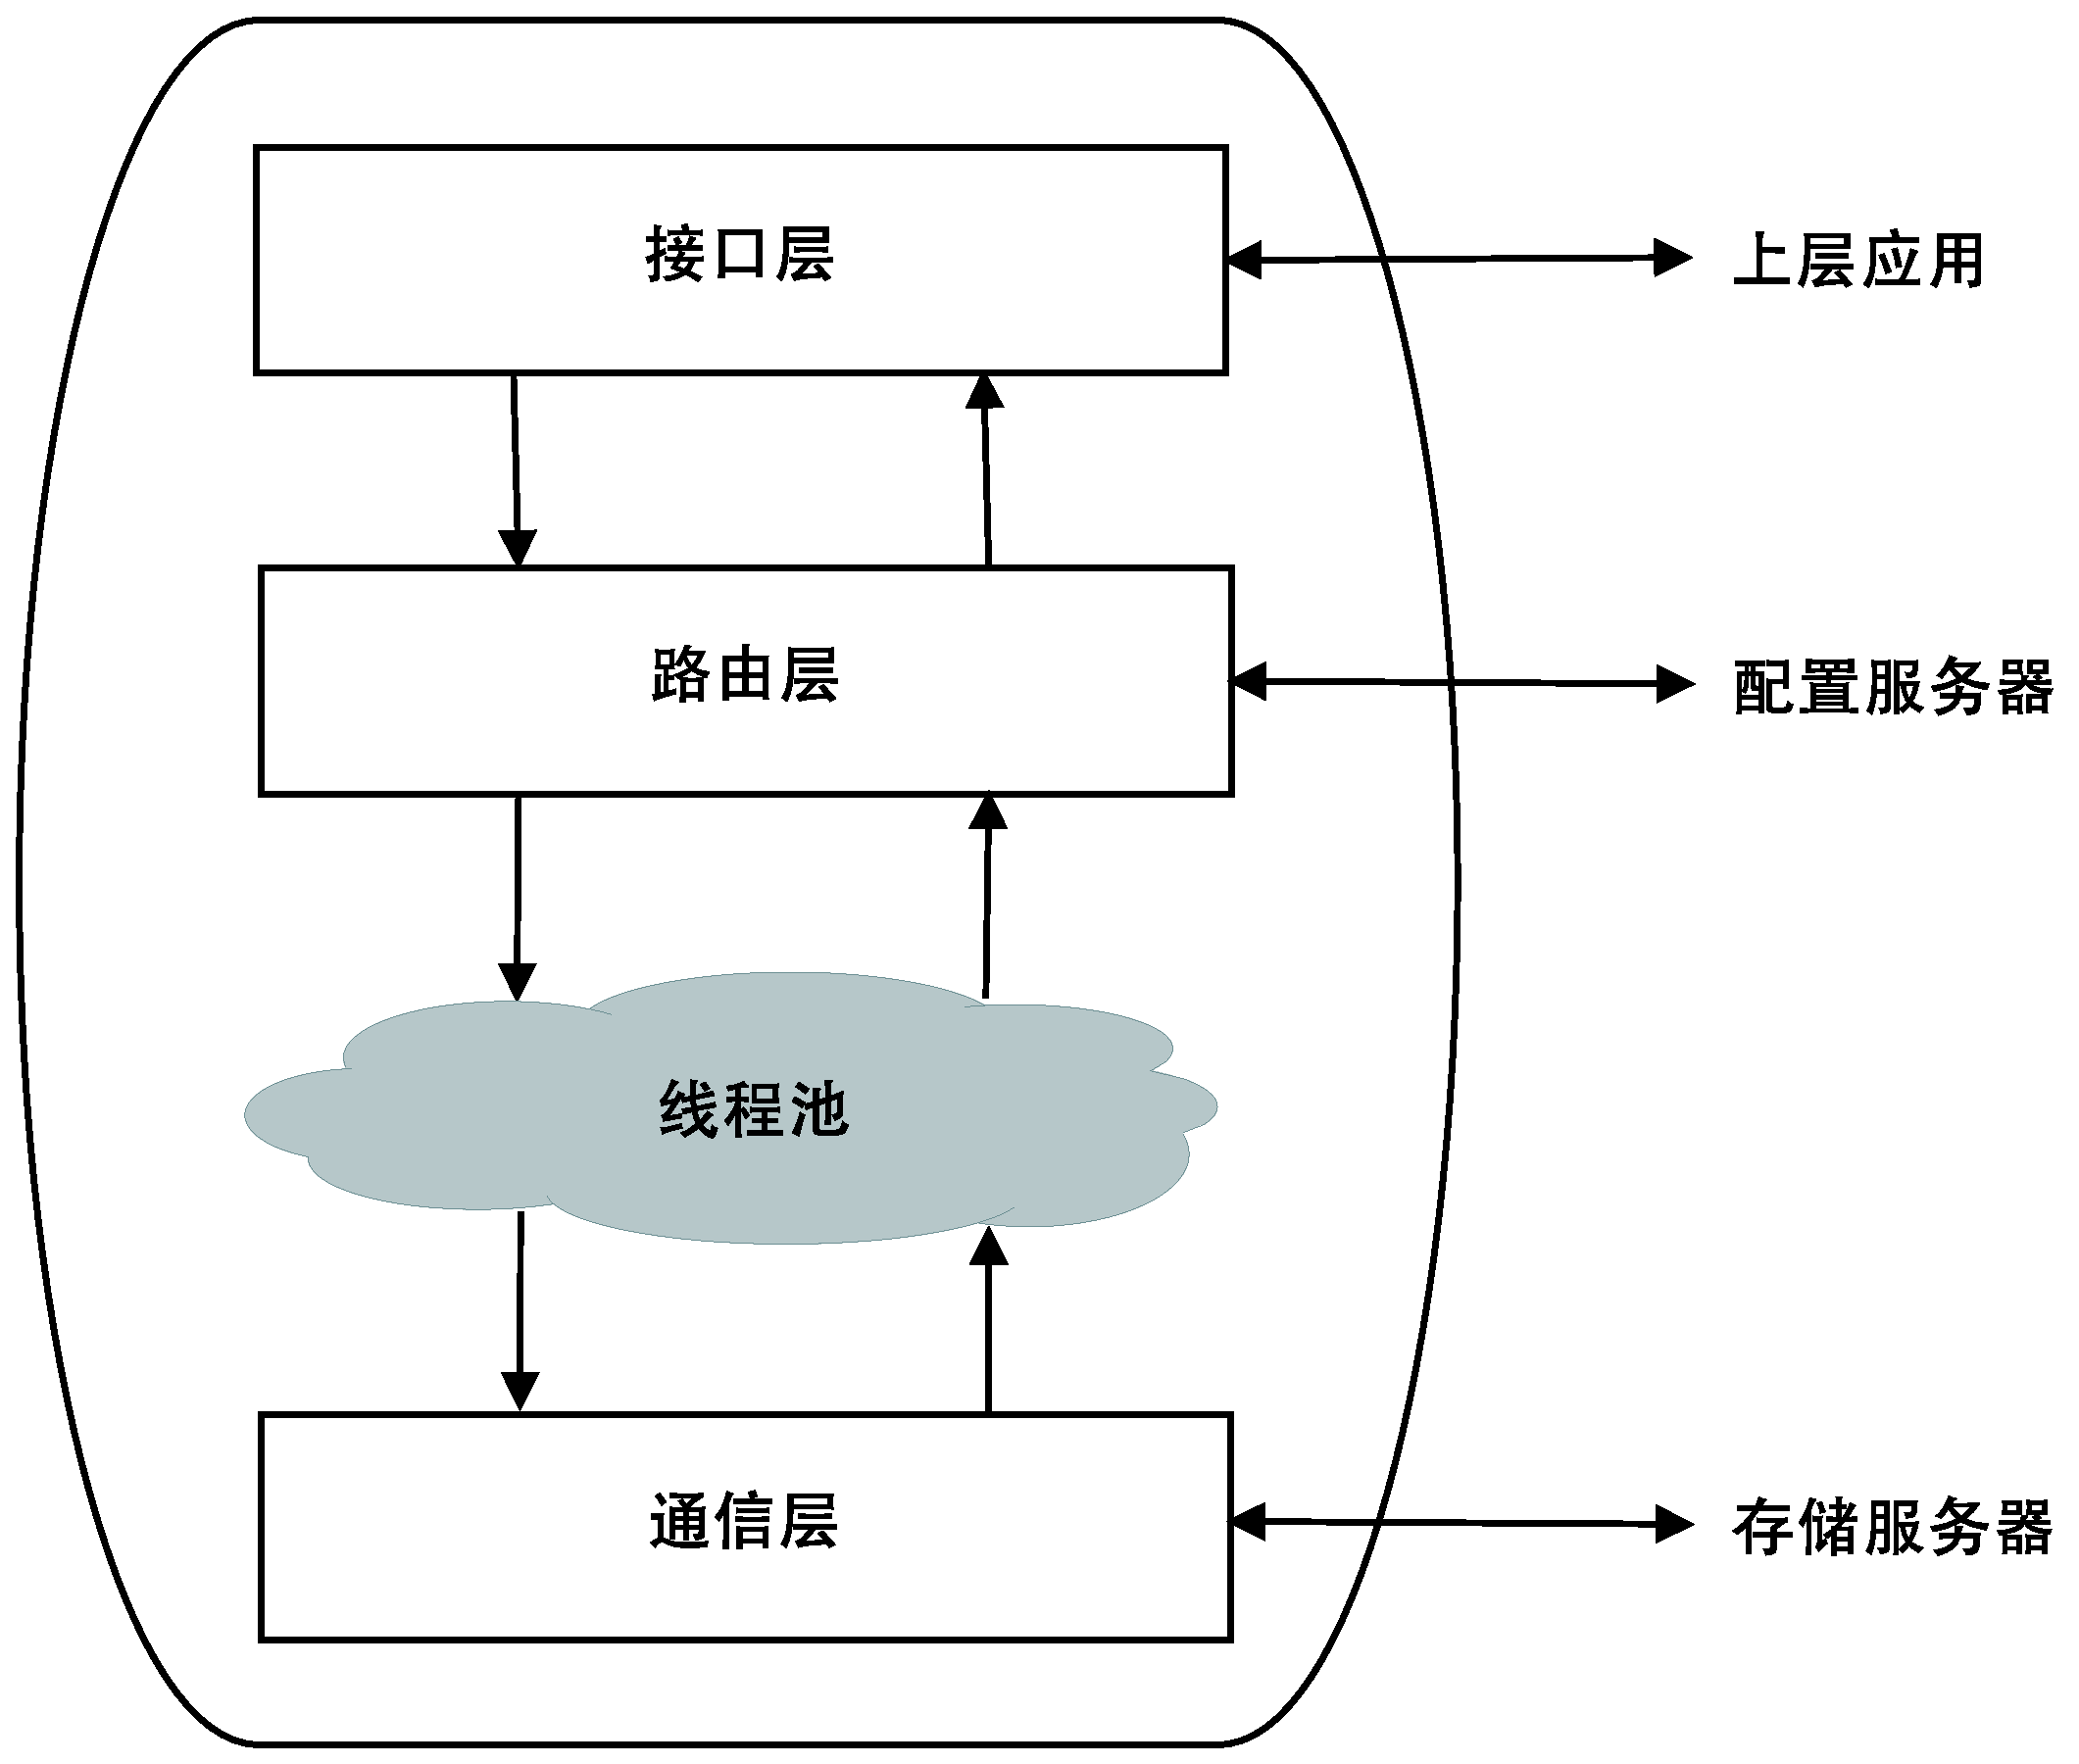
\includegraphics[width=0.8\linewidth]{client}
  \caption[分布式二级哈希表客户端]{分布式二级哈希表客户端。}
  \label{figure:client}
\end{figure}

\section{Redis}\label{section:redis}

\section{容错}\label{section:fault}

